\section*{Ejercicio 1}
\graphicspath{{Figuras/}}

Para este ejercicio se busco resolver el problema de XOR a partir de dos arquitecturas distintas, las cuales pueden observarse en la Figura \ref{fig:1_Arquitecturas} y cuya principal diferencia es que una presenta una reinyección de la entrada mientras que otra no. En ambos casos, la función de activación de la capa oculta fue $\tanh$ y como función de costo se utilizo MSE. Debido a que la función de activación utilizada nunca retorna $1$ o $-1$, se determino un umbral de 0.9 en la función de costo, de manera que si el resultado supera dicho umbral, se considera la salida como 1. De manera análoga, se determino un segundo umbral de -0.9 para determinar cuando la salida se considera un -1.

\begin{figure}[h!]
    \centering
    \begin{subfigure}[h]{0.3\textwidth} 
        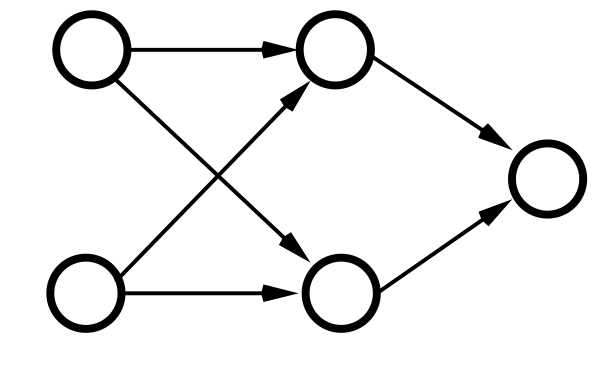
\includegraphics[width=\textwidth]{Figuras/ejer_1_221.png}
    \end{subfigure}       
    \begin{subfigure}[h]{0.3\textwidth} 
        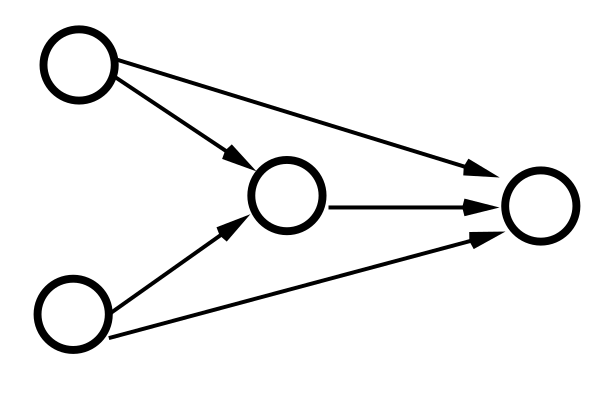
\includegraphics[width=\textwidth]{Figuras/ejer_1_211.png}
    \end{subfigure}
    \caption{Esquema de las arquitecturas utilizadas para resolver el problema del XOR.} \label{fig:1_Arquitecturas}
\end{figure}

En ambos casos se utilizo la totalidad de los datos como datos de entrenamiento. Los resultados para la función de costo y el \textit{accuracy} para la primer arquitectura en 10 procesos de entrenamiento independientes de la red pueden observarse en la Fig. \ref{fig:1_1erArquitectura}, mientras que en la Fig. \ref{fig:1_2daArquitectura} se observan los resultados análogos para la segunda arquitectura. En ambos casos se observa que algunos procesos de entrenamiento no convergen y no alcanzan un valor de \textit{accuracy} optimo del $100\%$.

\begin{figure}[h!]
    \centering
    \begin{subfigure}[h]{0.49\textwidth} 
        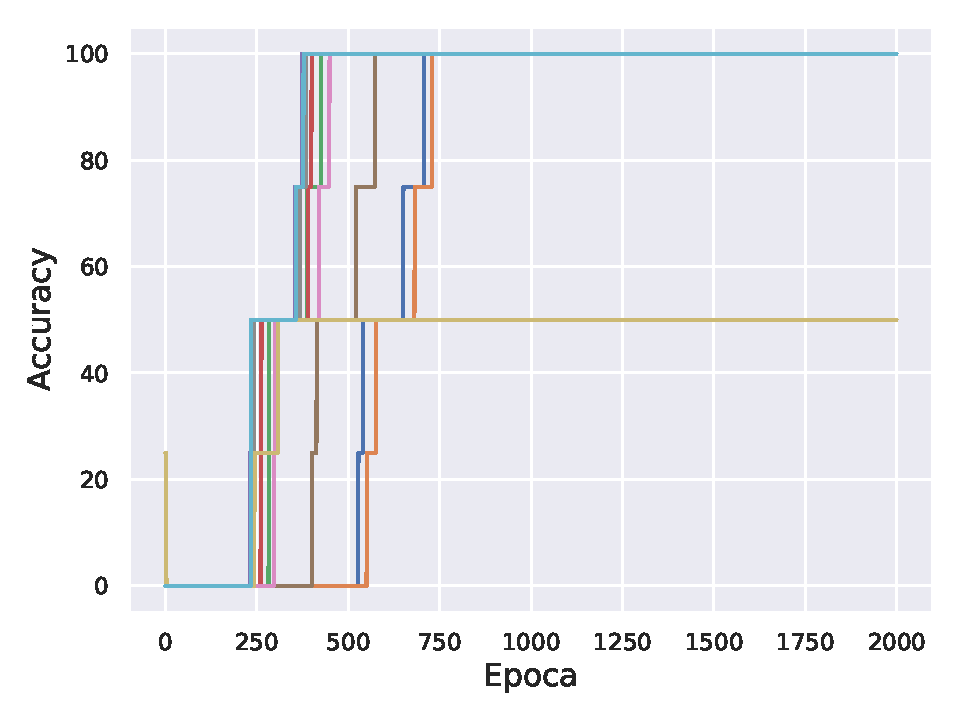
\includegraphics[width=\textwidth]{Figuras/ej1_1erArquitectura/Acc.pdf}
    \end{subfigure}       
    \begin{subfigure}[h]{0.49\textwidth} 
        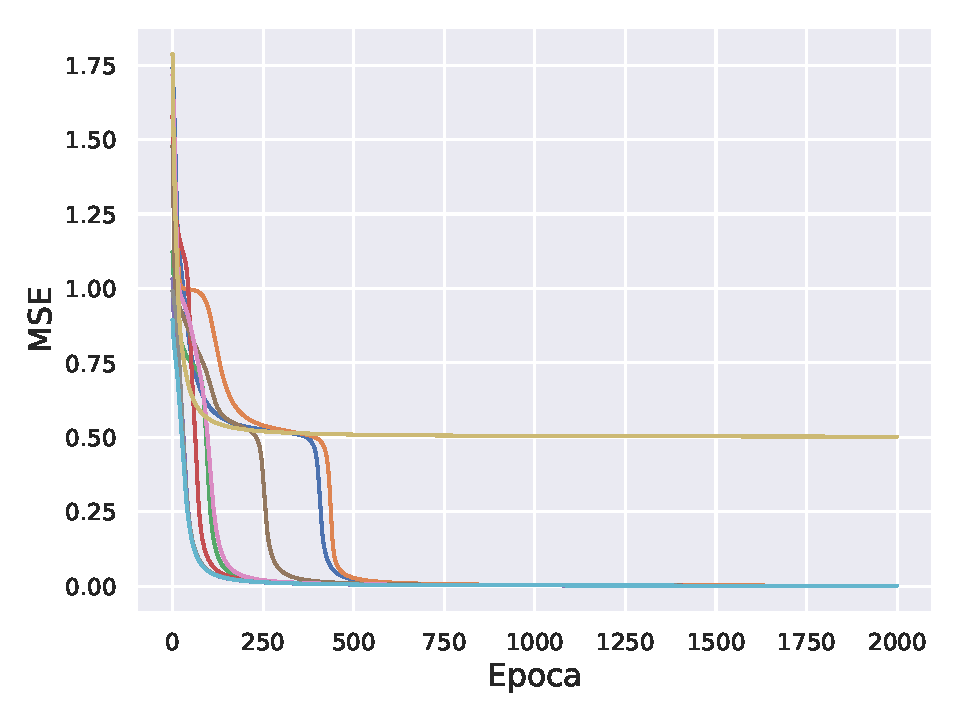
\includegraphics[width=\textwidth]{Figuras/ej1_1erArquitectura/Loss.pdf}
    \end{subfigure}
    \caption{Función de costo MSE y \textit{accuracy} para el entrenamiento de 10 modelos independientes, utilizando la primer arquitectura propuesta en Fig. \ref{fig:1_Arquitecturas}.} \label{fig:1_1erArquitectura}
\end{figure}

\begin{figure}[h!]
    \centering
    \begin{subfigure}[h]{0.49\textwidth} 
        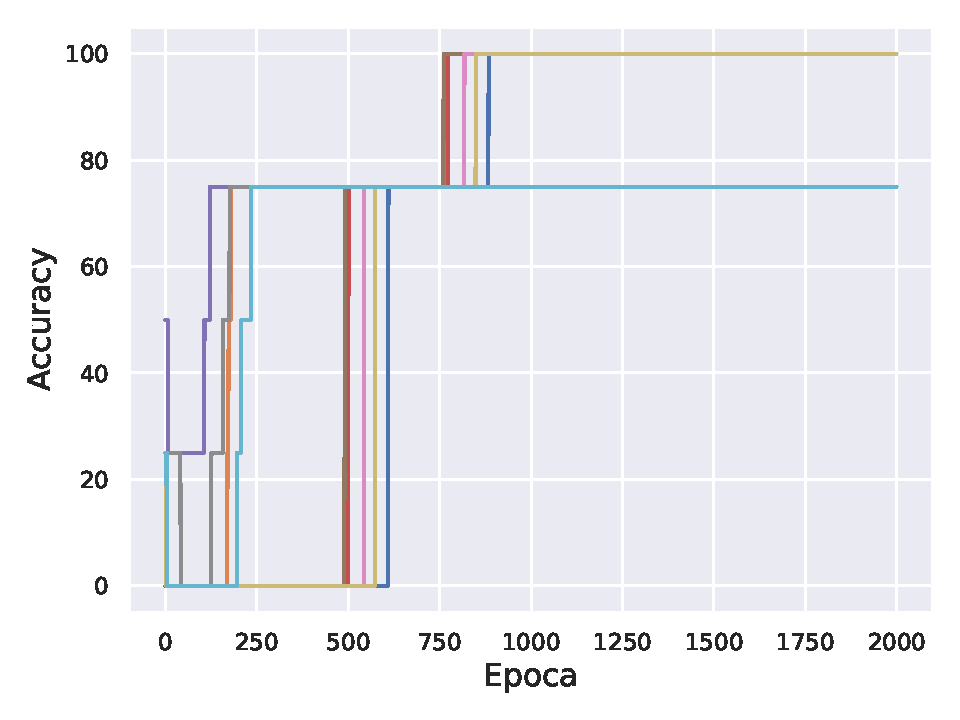
\includegraphics[width=\textwidth]{Figuras/ej1_2daArquitectura/Acc.pdf}
    \end{subfigure}       
    \begin{subfigure}[h]{0.49\textwidth} 
        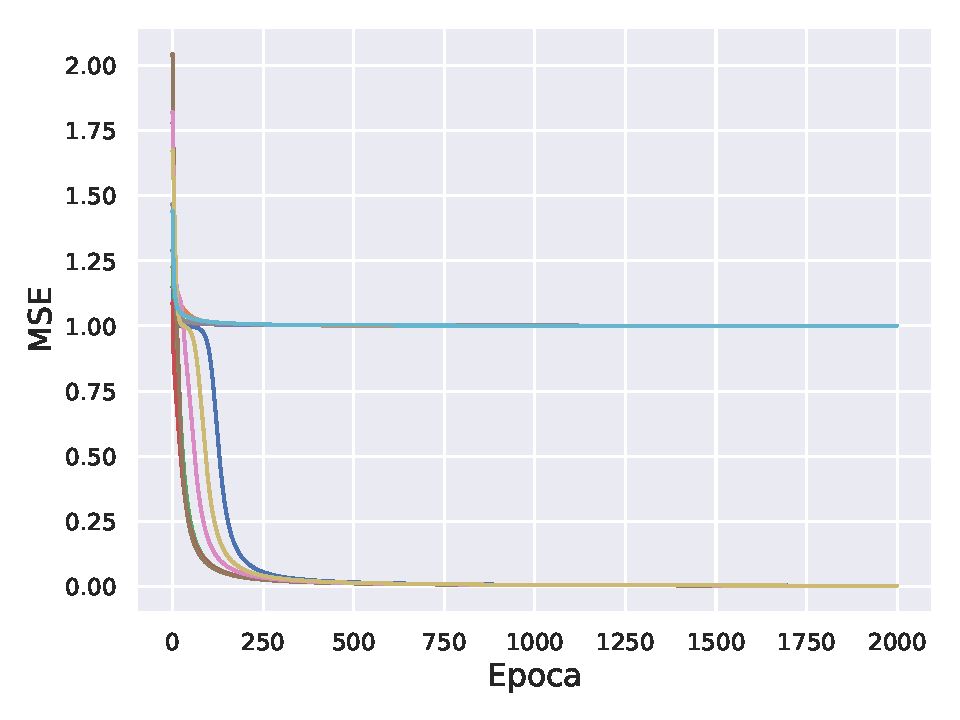
\includegraphics[width=\textwidth]{Figuras/ej1_2daArquitectura/Loss.pdf}
    \end{subfigure}
    \caption{Función de costo MSE y \textit{accuracy} para el entrenamiento de 10 modelos independientes, utilizando la segunda arquitectura propuesta en Fig. \ref{fig:1_Arquitecturas}.} \label{fig:1_2daArquitectura}
\end{figure}

Se definió el tiempo de convergencia como aquella época en donde la función de costo alcanza un valor de $0.1$, pero solo para los modelos que convergieron a una solución optima dentro de las $2000$ épocas. Para comparar los tiempos de convergencia entre ambas arquitecturas, se entrenaron 1000 modelos independientes que lograron converger y se obtuvo su tiempo de convergencia, para ambas arquitecturas. Para la primer arquitectura se obtuvo un tiempo de convergencia promedio de $157.5$ épocas, mientras que para la segunda se obtuvo un valor de $148.7$. En principio, esta diferencia, aunque sea pequeña, podría indicar que la segunda arquitectura es mejor para la resolución del problema XOR. Sin embargo, para obtener 1000 modelos entrenados que hayan logrado converger a una solución optima, fue necesario entrenar 1288 modelos para la primer arquitectura, mientras que para la segunda fueron necesarios 1983. Es decir, que el $77.6\%$ de los modelos creados con la primer arquitectura lograron converger, mientras que para la segunda solo el $50.4\%$, lo cual apunta a que la primer arquitectura es mas satisfactoria para resolver el problema.